\documentclass[twocolumn,11pt]{sotsuken_abst}




% タイトル
\title{1軸レーザ距離センサを用いたUAVの周辺認識についての研究}

\author{織田隆誠$\cdot$木村俊介$\cdot$村田涼真(指導教員 伊藤恒平)}

%\urlstyle{rm}

\setcounter{page}{13}
\lhead{}
\chead{}
\rhead{{\sf 12・207}\\{\bf 機械工学科}}
\lfoot{}
\cfoot{{\sf-\ M-\thepage \ -}}
%\rfoot{}
\renewcommand{\headrulewidth}{3pt}
%\renewcommand{\footrulewidth}{1pt}



\begin{document}
%\layout
\maketitle
\thispagestyle{fancy}
\pagestyle{fancy}

\setlength{\baselineskip}{5.6truemm}
\kanjiskip=.07zw plus 3pt minus 3pt
\xkanjiskip=.07zw plus 3pt minus 3pt


% 本文

\section{緒言}
\subsection{研究の背景}
近年無人航空機(Unmanned Aerial Vehicle:UAV)の研究と実用化に向けての動きが活発である.軍事目的では早い時期から実用化されており,民事でも農薬散布などの目的に実用化されている.さらに図\ref{fig:Quad.JPG}に示すようなマルチコプターの登場により研究開発が活性化してきており,様々な分野での活躍が期待されている.

\begin{figure}[htbp]
  \begin{center}
    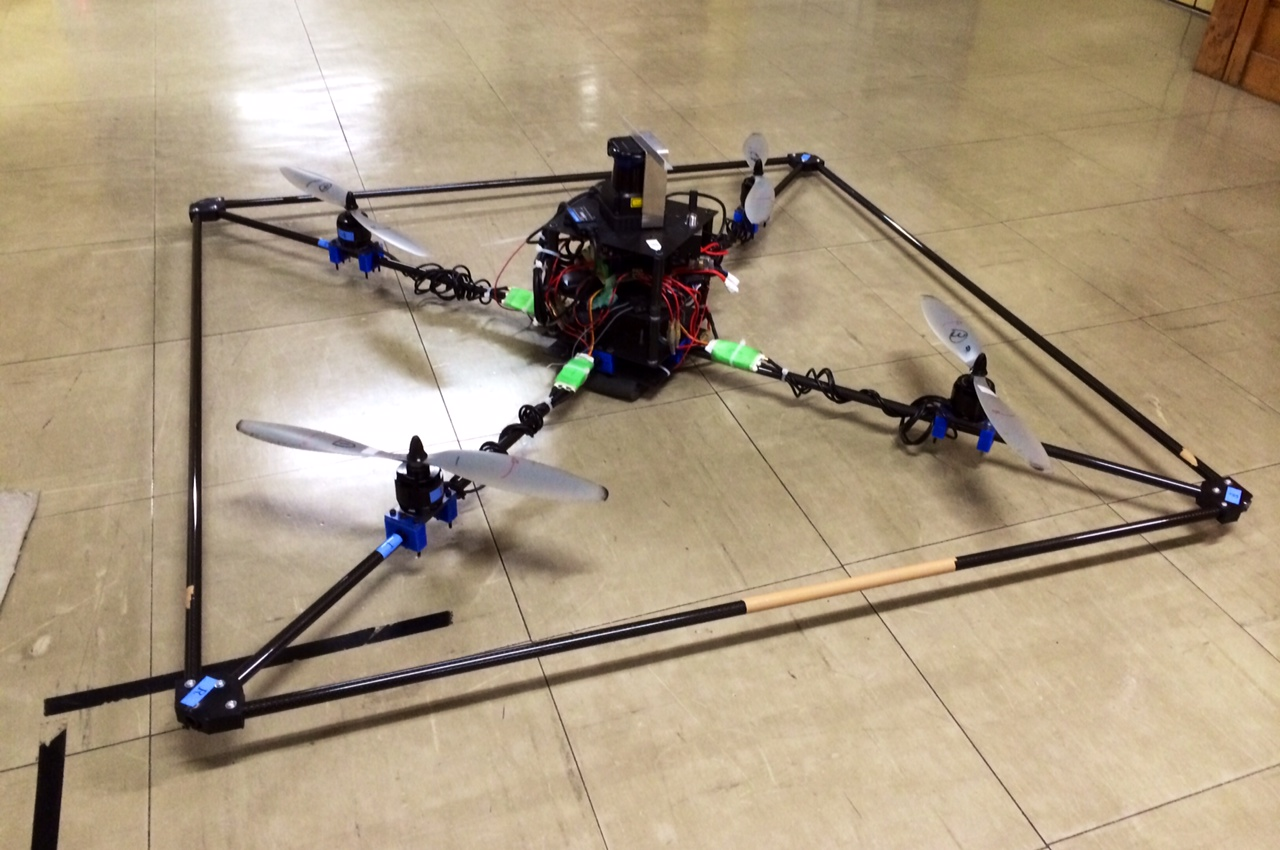
\includegraphics[width=60mm]{img/Quad.jpg}
    \end{center}
  \caption{実験に使用したクワッドロータ}
 \label{fig:Quad.JPG}
\end{figure}

\subsection{研究の目的}
UAVの活用の場として偵察,監視,空撮,地図作成,運搬等が考えられるがそれらは,UAVに適当なセンサを搭載し制御できることが求められる.しかしレーザスキャナを搭載するためには、その重量を運搬可能な機体が必要である.しかし,一般の空撮とそれに付属した地図作成の場合は比較的大型の機体を用いることができ、センサの重量、大きさはさほど問題にはならないが、仮に地図を作成しなければならない場所が屋内だとすれば、必然的にUAVの大きさの制限を受け,小型化を追求する事になる.このUAVの小型化という課題は今後UAVが活躍していく上で重要な項目である.
そこで筆者らはUAVに搭載するセンサの中で特に重要で重量が大きい,スキャン式レーザ距離計を,小型UAVに対応させるため軽量化した一軸レーザ距離計の試作を試みた.実験では一軸レーザセンサが自律飛行において情報収集能力があるかどうかを確認したので報告する.


\section{Quad Rotor}
我々は実験用のUAVとしてプロペラが4枚あるクアッドコプターを用いている.従来,筆者らの制作した機体はアルミ材を主としたため,機体重量が大きく軽量化が課題であった.そこで,フレーム材としてカーボン製のパイプや板,樹脂ブロックを使用し,試作機の重量を約半分に軽量化した.また,使用したブラシレスモータはT-Morter社製U5,バッテリは22.2V3300mAhを使用し,新型UAVは、手動操縦時での試験飛行ではホバリングを連続10分飛行することが出来る.

\section{一軸レーザ距離センサ}
UAVによる周辺状況の取得には,スキャン式レーザ距離計を用いるのが一般的である,しかしUAVの軽量化を目標としたときに,筆者らは,大きな重量を要するスキャン機構を取り除くことで実現することとした.
スキャン式レーザ距離計は内部の基準板を観測することにより熱的な変動を校正していたが,制作したセンサはスキャンをしないため基準板を見ることができないためこの手法は用いることが出来ない.そこで,元となったセンサに備わっていたマルチエコー機能を用いて距離既知の基準板を第1エコーが帰る場所に置き,第2エコーは被計測物から帰ってくるものとして,熱的な変動を低減することができた.使用する1軸レーザ距離センサを図\ref{fig:sensor.png}に示す.

\begin{figure}[htbp]
  \begin{center}
    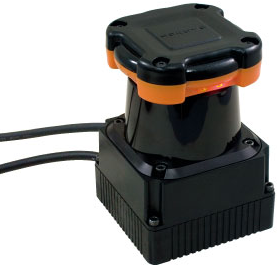
\includegraphics[width=60mm]{img/sensor.png}
    \end{center}
  \caption{実験に使用した1軸レーザ距離センサ}
 \label{fig:sensor.png}
\end{figure}

\section{壁沿い飛行について}
UAVは一軸レーザ距離センサ搭載であるので,両側の壁と進行方向にあると思われる障害物の認識をセンサで読み取りながら進んでく.通常のスキャン式レーザ距離計であれば周辺状況を瞬時に取得可能であるが,一軸レーザ距離計では不可能であるので以下の壁沿い飛行方式を考えている.
壁と進行方向にある障害物をセンサで読み取りながら進み,障害物を発見した場合,回避するために前後もしくは横移動する.同様の行動を繰り返し移動する.
以上の方法を図\ref{fig:5.png}に示す.

\begin{figure}[htbp]
  \begin{center}
    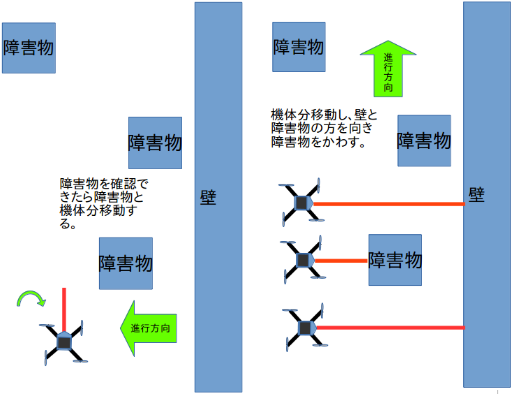
\includegraphics[width=60mm]{img/5.png}
    \end{center}
  \caption{壁沿い飛行の構想}
 \label{fig:5.png}
\end{figure}

\section{周辺状況の取得実験}
1軸レーザ距離センサが有効で実際に使用できるか確認するために周辺状況の取得実験を行う.実験方法はUAVを図のように固定し,手動とコントローラーを使い低速・中速・高速とそれぞれの速さで固定されているUAVを回転させ,速さの違いでセンサがどのように読み取りを行うかを実験した.実験装置を図\ref{fig:7.png}に示す.取得環境を図\ref{fig:kankyou.png}に示す.取得した結果を図\ref{fig:keka1.png}に示す.実験結果よりおおむね周辺環境の取得が可能であることがわかった.

\begin{figure}[htbp]
  \begin{center}
    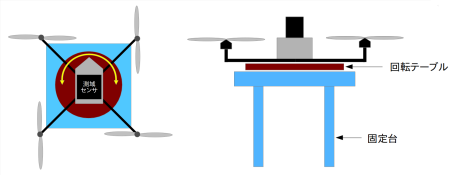
\includegraphics[width=60mm]{img/7.png}
    \end{center}
  \caption{周辺状況の取得実験}
 \label{fig:7.png}
\end{figure}

\begin{figure}[htbp]
  \begin{center}
    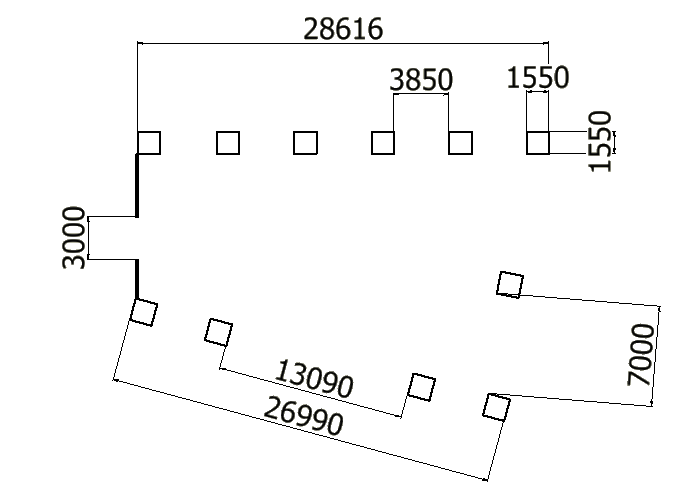
\includegraphics[width=60mm]{img/kankyou.png}
    \end{center}
  \caption{取得環境}
 \label{fig:kankyou.png}
\end{figure}

\begin{figure}[htbp]
  \begin{center}
    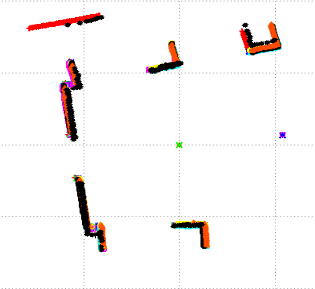
\includegraphics[width=60mm]{img/keka1.png}
    \end{center}
  \caption{実験結果}
 \label{fig:keka1.png}
\end{figure}

\section{結言}
小型UAVに搭載する軽量化した一軸レーザーセンサを用いた壁沿い飛行を行う機体の実現にあたり,一軸センサでの周辺状況の取得について実験により有効性を確認した.一軸センサの特性上,センサ正面の距離を測定する事しかできず,左右の障害物を特定するためには実際に機体がそちらの方向を向き、計測しながら移動する必要があった.そこで機体をゆっくり一周させて周辺状況を取得する実験を試みたが,実験の結果一軸レーザーセンサによる周辺状況の取得は成功した.
災害現場などで活躍するにはより、複雑な地形を読み取り対応する必要がある.今後は実際に飛行プログラムと連携し取得したデータを用いながら移動する手法の検討にはいる予定である.

% 参考文献
\begin{thebibliography}{8}
%  \bibitem{harris} LandingProducts, APCPro\nolinebreak pellers,\nolinebreak
%http://www.\linebreak apcprop. com{\slash}v{\slash}index.html,
%2012/8/21
\bibitem{ros} WillowGarage,AboutROS,http://www.ros.org/\linebreak about-ros/, 2013/12/18
%  \bibitem{kyonenn} 東 勇樹,岩本健太,安田瑞規:クワッドロータ飛行ロボット製作における模型用プロペラの選定,1D12,第50回飛行機シンポジウム,新潟,2012
%  \bibitem{koukuu} 中村 資郎:新航空工学講座 第7巻 プロペラ:日本航空技術協会,pp.23-24,1988
%  \bibitem{rikigaku} 加藤 寛一郎,大屋 昭男,柄沢 研治:航空機力学入門,東京大学出版会,pp.32,1982
\end{thebibliography}


\end{document}

○○○○○○○○○○○○○○○○○○○○○○○○○○○○○○○○○○○○○○○○○○○○○○○○
○○○○○○○○○○○○○○○○○○○○○○○○○○○○○○○○○○○○○○○○○○○○○○○○
○○○○○○○○○○○○○○○○○○○○○○○○○○○○○○○○○○○○○○○○○○○○○○○○
○○○○○○○○○○○○○○○○○○○○○○○○○○○○○○○○○○○○○○○○○○○○○○○○
○○○○○○○○○○○○○○○○○○○○○○○○○○○○○○○○○○○○○○○○○○○○○○○○
○○○○○○○○○○○○○○○○○○○○○○○○○○○○○○○○○○○○○○○○○○○○○○○○
○○○○○○○○○○○○○○○○○○○○○○○○○○○○○○○○○○○○○○○○○○○○○○○○
○○○○○○○○○○○○○○○○○○○○○○○○○○○○○○○○○○○○○○○○○○○○○○○○
○○○○○○○○○○○○○○○○○○○○○○○○○○○○○○○○○○○○○○○○○○○○○○○○
○○○○○○○○○○○○○○○○○○○○○○○○○○○○○○○○○○○○○○○○○○○○○○○○
○○○○○○○○○○○○○○○○○○○○○○○○○○○○○○○○○○○○○○○○○○○○○○○○
○○○○○○○○○○○○○○○○○○○○○○○○○○○○○○○○○○○○○○○○○○○○○○○○
○○○○○○○○○○○○○○○○○○○○○○○○○○○○○○○○○○○○○○○○○○○○○○○○
○○○○○○○○○○○○○○○○○○○○○○○○○○○○○○○○○○○○○○○○○○○○○○○○
○○○○○○○○○○○○○○○○○○○○○○○○○○○○○○○○○○○○○○○○○○○○○○○○
○○○○○○○○○○○○○○○○○○○○○○○○○○○○○○○○○○○○○○○○○○○○○○○○
○○○○○○○○○○○○○○○○○○○○○○○○○○○○○○○○○○○○○○○○○○○○○○○○
○○○○○○○○○○○○○○○○○○○○○○○○○○○○○○○○○○○○○○○○○○○○○○○○
○○○○○○○○○○○○○○○○○○○○○○○○○○○○○○○○○○○○○○○○○○○○○○○○
○○○○○○○○○○○○○○○○○○○○○○○○○○○○○○○○○○○○○○○○○○○○○○○○
○○○○○○○○○○○○○○○○○○○○○○○○○○○○○○○○○○○○○○○○○○○○○○○○
○○○○○○○○○○○○○○○○○○○○○○○○○○○○○○○○○○○○○○○○○○○○○○○○
○○○○○○○○○○○○○○○○○○○○○○○○○○○○○○○○○○○○○○○○○○○○○○○○
○○○○○○○○○○○○○○○○○○○○○○○○○○○○○○○○○○○○○○○○○○○○○○○○
○○○○○○○○○○○○○○○○○○○○○○○○○○○○○○○○○○○○○○○○○○○○○○○○
○○○○○○○○○○○○○○○○○○○○○○○○○○○○○○○○○○○○○○○○○○○○○○○○
○○○○○○○○○○○○○○○○○○○○○○○○○○○○○○○○○○○○○○○○○○○○○○○○
○○○○○○○○○○○○○○○○○○○○○○○○○○○○○○○○○○○○○○○○○○○○○○○○
○○○○○○○○○○○○○○○○○○○○○○○○○○○○○○○○○○○○○○○○○○○○○○○○
○○○○○○○○○○○○○○○○○○○○○○○○○○○○○○○○○○○○○○○○○○○○○○○○
○○○○○○○○○○○○○○○○○○○○○○○○○○○○○○○○○○○○○○○○○○○○○○○○
○○○○○○○○○○○○○○○○○○○○○○○○○○○○○○○○○○○○○○○○○○○○○○○○
○○○○○○○○○○○○○○○○○○○○○○○○○○○○○○○○○○○○○○○○○○○○○○○○
○○○○○○○○○○○○○○○○○○○○○○○○○○○○○○○○○○○○○○○○○○○○○○○○
○○○○○○○○○○○○○○○○○○○○○○○○○○○○○○○○○○○○○○○○○○○○○○○○
○○○○○○○○○○○○○○○○○○○○○○○○○○○○○○○○○○○○○○○○○○○○○○○○
○○○○○○○○○○○○○○○○○○○○○○○○○○○○○○○○○○○○○○○○○○○○○○○○
○○○○○○○○○○○○○○○○○○○○○○○○○○○○○○○○○○○○○○○○○○○○○○○○
○○○○○○○○○○○○○○○○○○○○○○○○○○○○○○○○○○○○○○○○○○○○○○○○
○○○○○○○○○○○○○○○○○○○○○○○○○○○○○○○○○○○○○○○○○○○○○○○○
○○○○○○○○○○○○○○○○○○○○○○○○○○○○○○○○○○○○○○○○○○○○○○○○
○○○○○○○○○○○○○○○○○○○○○○○○○○○○○○○○○○○○○○○○○○○○○○○○
○○○○○○○○○○○○○○○○○○○○○○○○○○○○○○○○○○○○○○○○○○○○○○○○
○○○○○○○○○○○○○○○○○○○○○○○○○○○○○○○○○○○○○○○○○○○○○○○○
○○○○○○○○○○○○○○○○○○○○○○○○○○○○○○○○○○○○○○○○○○○○○○○○
○○○○○○○○○○○○○○○○○○○○○○○○○○○○○○○○○○○○○○○○○○○○○○○○
○○○○○○○○○○○○○○○○○○○○○○○○○○○○○○○○○○○○○○○○○○○○○○○○
○○○○○○○○○○○○○○○○○○○○○○○○○○○○○○○○○○○○○○○○○○○○○○○○
○○○○○○○○○○○○○○○○○○○○○○○○○○○○○○○○○○○○○○○○○○○○○○○○
○○○○○○○○○○○○○○○○○○○○○○○○○○○○○○○○○○○○○○○○○○○○○○○○
○○○○○○○○○○○○○○○○○○○○○○○○○○○○○○○○○○○○○○○○○○○○○○○○
○○○○○○○○○○○○○○○○○○○○○○○○○○○○○○○○○○○○○○○○○○○○○○○○
○○○○○○○○○○○○○○○○○○○○○○○○○○○○○○○○○○○○○○○○○○○○○○○○
○○○○○○○○○○○○○○○○○○○○○○○○○○○○○○○○○○○○○○○○○○○○○○○○
○○○○○○○○○○○○○○○○○○○○○○○○○○○○○○○○○○○○○○○○○○○○○○○○
○○○○○○○○○○○○○○○○○○○○○○○○○○○○○○○○○○○○○○○○○○○○○○○○
○○○○○○○○○○○○○○○○○○○○○○○○○○○○○○○○○○○○○○○○○○○○○○○○
○○○○○○○○○○○○○○○○○○○○○○○○○○○○○○○○○○○○○○○○○○○○○○○○
○○○○○○○○○○○○○○○○○○○○○○○○○○○○○○○○○○○○○○○○○○○○○○○○
○○○○○○○○○○○○○○○○○○○○○○○○○○○○○○○○○○○○○○○○○○○○○○○○
○○○○○○○○○○○○○○○○○○○○○○○○○○○○○○○○○○○○○○○○○○○○○○○○
○○○○○○○○○○○○○○○○○○○○○○○○○○○○○○○○○○○○○○○○○○○○○○○○
○○○○○○○○○○○○○○○○○○○○○○○○○○○○○○○○○○○○○○○○○○○○○○○○
○○○○○○○○○○○○○○○○○○○○○○○○○○○○○○○○○○○○○○○○○○○○○○○○
○○○○○○○○○○○○○○○○○○○○○○○○○○○○○○○○○○○○○○○○○○○○○○○○
○○○○○○○○○○○○○○○○○○○○○○○○○○○○○○○○○○○○○○○○○○○○○○○○
○○○○○○○○○○○○○○○○○○○○○○○○○○○○○○○○○○○○○○○○○○○○○○○○
○○○○○○○○○○○○○○○○○○○○○○○○○○○○○○○○○○○○○○○○○○○○○○○○
○○○○○○○○○○○○○○○○○○○○○○○○○○○○○○○○○○○○○○○○○○○○○○○○
○○○○○○○○○○○○○○○○○○○○○○○○○○○○○○○○○○○○○○○○○○○○○○○○
○○○○○○○○○○○○○○○○○○○○○○○○○○○○○○○○○○○○○○○○○○○○○○○○
○○○○○○○○○○○○○○○○○○○○○○○○○○○○○○○○○○○○○○○○○○○○○○○○
○○○○○○○○○○○○○○○○○○○○○○○○○○○○○○○○○○○○○○○○○○○○○○○○
○○○○○○○○○○○○○○○○○○○○○○○○○○○○○○○○○○○○○○○○○○○○○○○○
○○○○○○○○○○○○○○○○○○○○○○○○○○○○○○○○○○○○○○○○○○○○○○○○
○○○○○○○○○○○○○○○○○○○○○○○○○○○○○○○○○○○○○○○○○○○○○○○○
○○○○○○○○○○○○○○○○○○○○○○○○○○○○○○○○○○○○○○○○○○○○○○○○
○○○○○○○○○○○○○○○○○○○○○○○○○○○○○○○○○○○○○○○○○○○○○○○○
○○○○○○○○○○○○○○○○○○○○○○○○○○○○○○○○○○○○○○○○○○○○○○○○
○○○○○○○○○○○○○○○○○○○○○○○○○○○○○○○○○○○○○○○○○○○○○○○○
○○○○○○○○○○○○○○○○○○○○○○○○○○○○○○○○○○○○○○○○○○○○○○○○
○○○○○○○○○○○○○○○○○○○○○○○○○○○○○○○○○○○○○○○○○○○○○○○○
○○○○○○○○○○○○○○○○○○○○○○○○○○○○○○○○○○○○○○○○○○○○○○○○
○○○○○○○○○○○○○○○○○○○○○○○○○○○○○○○○○○○○○○○○○○○○○○○○
○○○○○○○○○○○○○○○○○○○○○○○○○○○○○○○○○○○○○○○○○○○○○○○○
○○○○○○○○○○○○○○○○○○○○○○○○○○○○○○○○○○○○○○○○○○○○○○○○
○○○○○○○○○○○○○○○○○○○○○○○○○○○○○○○○○○○○○○○○○○○○○○○○
○○○○○○○○○○○○○○○○○○○○○○○○○○○○○○○○○○○○○○○○○○○○○○○○
○○○○○○○○○○○○○○○○○○○○○○○○○○○○○○○○○○○○○○○○○○○○○○○○
○○○○○○○○○○○○○○○○○○○○○○○○○○○○○○○○○○○○○○○○○○○○○○○○
○○○○○○○○○○○○○○○○○○○○○○○○○○○○○○○○○○○○○○○○○○○○○○○○
○○○○○○○○○○○○○○○○○○○○○○○○○○○○○○○○○○○○○○○○○○○○○○○○
○○○○○○○○○○○○○○○○○○○○○○○○○○○○○○○○○○○○○○○○○○○○○○○○
○○○○○○○○○○○○○○○○○○○○○○○○○○○○○○○○○○○○○○○○○○○○○○○○
○○○○○○○○○○○○○○○○○○○○○○○○○○○○○○○○○○○○○○○○○○○○○○○○
○○○○○○○○○○○○○○○○○○○○○○○○○○○○○○○○○○○○○○○○○○○○○○○○
○○○○○○○○○○○○○○○○○○○○○○○○○○○○○○○○○○○○○○○○○○○○○○○○
○○○○○○○○○○○○○○○○○○○○○○○○○○○○○○○○○○○○○○○○○○○○○○○○
○○○○○○○○○○○○○○○○○○○○○○○○○○○○○○○○○○○○○○○○○○○○○○○○
○○○○○○○○○○○○○○○○○○○○○○○○○○○○○○○○○○○○○○○○○○○○○○○○
○○○○○○○○○○○○○○○○○○○○○○○○○○○○○○○○○○○○○○○○○○○○○○○○
○○○○○○○○○○○○○○○○○○○○○○○○○○○○○○○○○○○○○○○○○○○○○○○○
○○○○○○○○○○○○○○○○○○○○○○○○○○○○○○○○○○○○○○○○○○○○○○○○
○○○○○○○○○○○○○○○○○○○○○○○○○○○○○○○○○○○○○○○○○○○○○○○○


